\section{Cross-Validation (CV)}

\begin{itemize}
    \item a technique to compare (and select from) different models (=different parameter values)
    \item Use case 1: Obtain a better estimate of the generalization error
    \item Use case 2: Selection of hyper parameters, split/train pattern of cross validation can be used to find optimal hyper parameters
\end{itemize}

\textbf{Problem with (80/20) Data Separation}
\begin{itemize}
    \item Test Error depends on random set
    \item For different sets, the test error would be different
\end{itemize}

without cross-validation

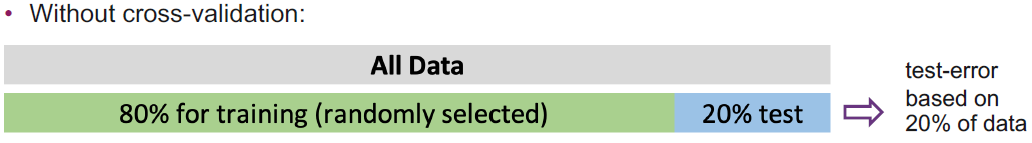
\includegraphics[width=\linewidth]{k_fold.png}

\subsection{k-fold Cross-Validation}

With k-Fold Cross-Validation\\

\begin{itemize}
    \item The data is split once into k folds
    \item Repeats the split-train-test procedure k times, using a systematic resampling procedure
    \item Then train/test is repeated k-times.
    \item Each fold participates in k-1 training phases and is used once for testing
\end{itemize}

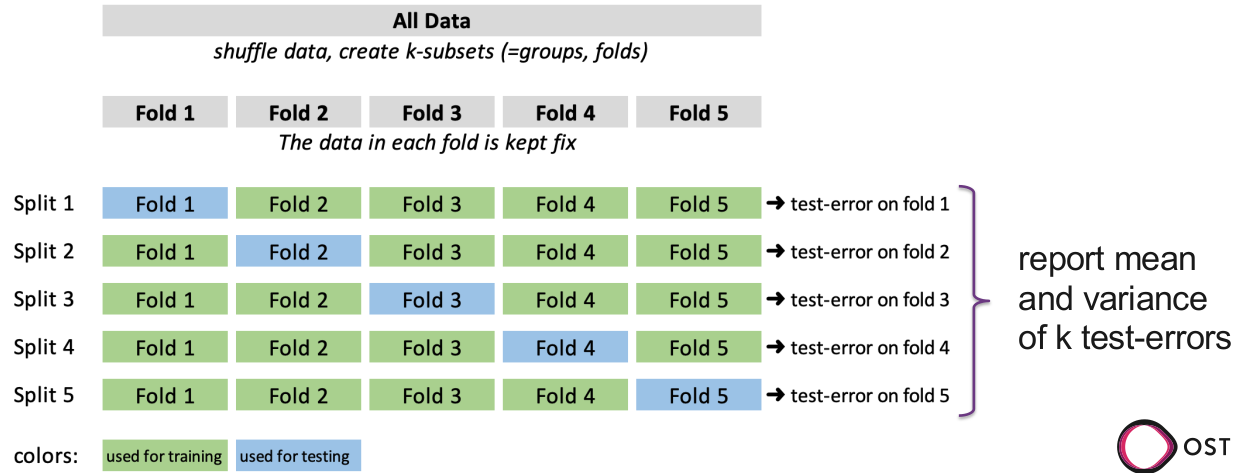
\includegraphics[width=\linewidth]{k_fold2.png}

\begin{itemize}
    \item Typical Values for k are 5,10 or N
    \item The data of a fold does not change during procedure
    \item Do not preprocess the whole dataset
    \item Apply the preprocessing pipeline (standardization) to each split
    \item Each split generates a different model
    \item With regularization, each split may yield a different  model and a different optimal $\lambda$
\end{itemize}

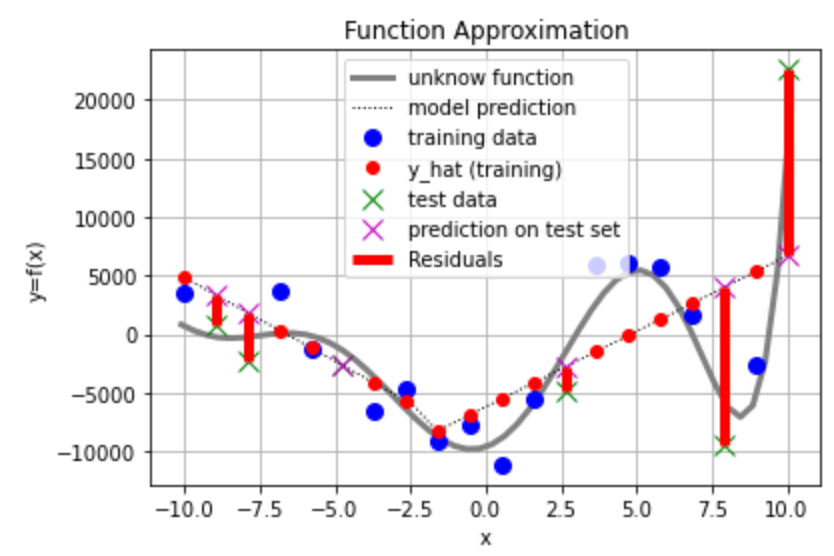
\includegraphics[width=\linewidth]{learning-model.png}

\textbf{Compare results}

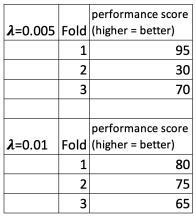
\includegraphics[width=0.5\linewidth]{compare-folds.png}

$220/3 > 195/3$ results in better regularization of $\lambda = 0.01$
